\documentclass[letterpaper]{article}

\usepackage{graphicx}
\usepackage[letterpaper, left=30mm, right=30mm, top=30mm, bottom=30mm]{geometry}

\begin{document}

\begin{flushright}
	
\includegraphics[width=5cm, height=4cm]{logoMATCOM.png}\\
	{\scriptsize \textbf{Facultad de Matemática y Computación}}
\end{flushright}

\

\

\begin{center}
	\textbf{{\Huge PROYECTO DE }}
	
	\

	\textbf{{\Huge PROGRAMACIÓN I}}
	\

	\

	\

	\

	\

	\textbf{{\Huge Moogle!}}
\end{center}
\begin{figure}[b]
	\begin{flushleft}
		{\huge \textbf{Estudiante:} \textit{Claudia Hernández Pérez}}

		\
	
		{\LARGE \textbf{Grupo:} \textit{C-122}}
	\end{flushleft}
\end{figure}

\newpage
{\small
El proyecto consta de 6 clases funcionales y una adicional con contenido relacionado con el
curso de Álgebra I sobre operaciones con matrices. A continuación se dispone a explicar dichas
clases:\\

\textbf{{\large- Process Documents}}\\

Esta clase se encarga de procesar los documentos de la base de datos antes de comenzar la
búsqueda. Se llama al método en la línea anterior a app.Run () para realizar esta operación una
sola vez antes de que arranque el programa y esté listo para ejecutarse (fig 1.1).

\begin{center}
	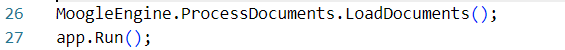
\includegraphics[width=8cm, height=0.75cm]{fig 1.1.png}\\
	{\tiny Fig. 1.1 Líneas de la clase Program de la carpeta MoogleServer}
\end{center}

{\normalsize¿Pero a qué le llamamos “procesar los documentos”?}

\begin{center}
	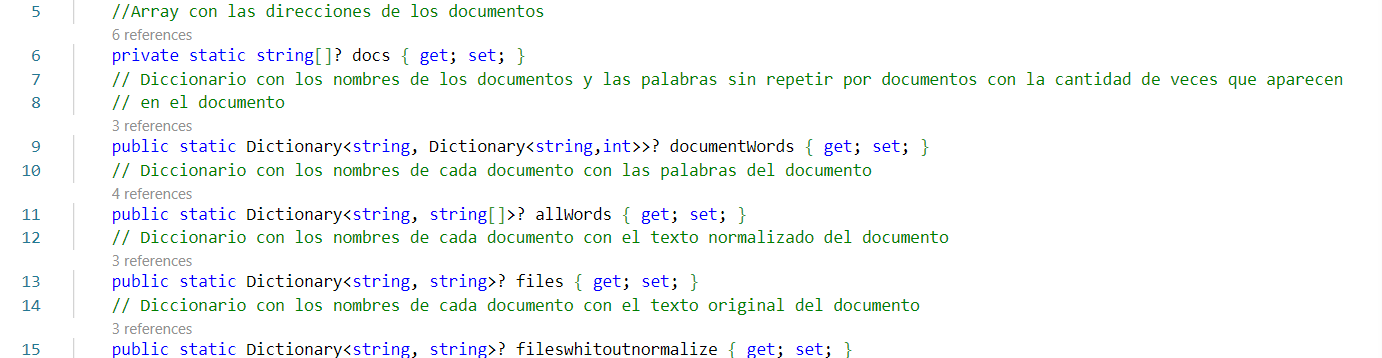
\includegraphics[width=11cm, height=3cm]{fig 1.2.png}\\
	{\tiny Fig. 1.2 Líneas de la clase ProcessDocuments de la carpeta MoogleEngine}
\end{center}

Primeramente, se accede al contenido de la carpeta “Content” (que estará dentro de la
carpeta moogle-main), independientemente de la ubicación en el dispositivo de la carpeta
moogle-main, se guardan las direcciones de los documentos en el array docs y con esta
información se acceden a los nombres de cada documento con la función predeterminada
Path.GetFileNameWithoutExtension (string path) y al texto de cada documento con
File.ReadAllText (string path). Con el cuerpo del documento y con la función
string.Split (string separator) se crea un array donde cada posición es una palabra. Luego
con estos datos guardados, en un ciclo foreach, se itera cada palabra por documento para
determinar la cantidad de veces que aparece (fig. 1.2).\\

\textbf{{\large- Documents}}\\

Esta clase está dirigida al trabajo con los documentos, se “normalizan”. Es decir, en caso de
que las búsquedas se realicen en español, se eliminan las tildes para evitar errores ortográficos.
Además, independientemente del idioma, se eliminan los signos de puntuación y cualquier otro
símbolo ajeno al alfabeto (de la “a” hasta la “z”, incluyendo la “ñ”) y los números (fig. 1.3).\\

\begin{center}
	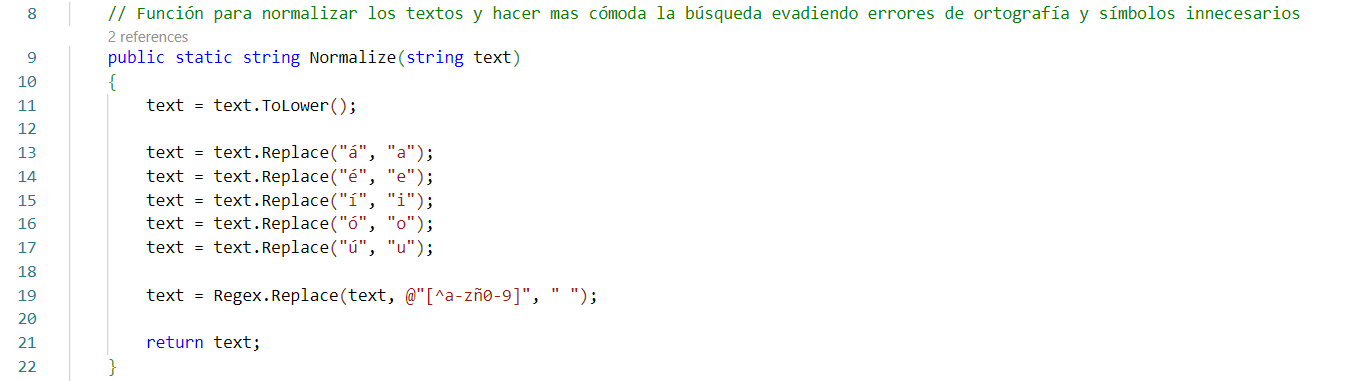
\includegraphics[width=11cm, height=3cm]{fig 1.3.png}\\
	{\tiny Fig. 1.3 Líneas de la clase Documents de la carpeta MoogleEngine}
\end{center}

Se encuentra además esta otra función para seleccionar el “snippet” (pedazo breve de
un texto), que se explicará su funcionamiento (fig. 1.4).
\begin{center}
	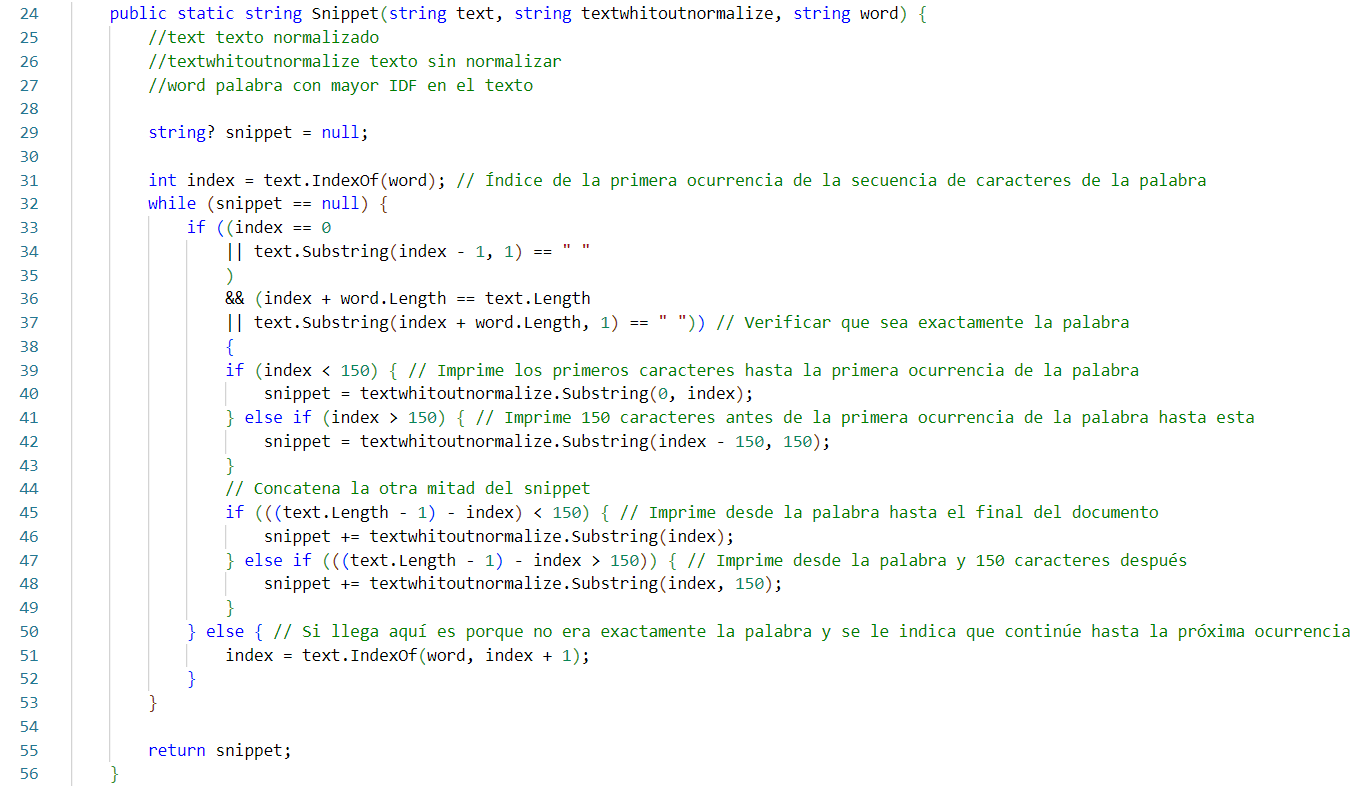
\includegraphics[width=12cm, height=6cm]{fig 1.4.png}\\
	{\tiny Fig. 1.4 Líneas de la clase Documents de la carpeta MoogleEngine}
\end{center}

Con la función string.IndexOf (string word) se busca la ocurrencia de la secuencia de
caracteres que se pase como parámetro, que en este caso es la palabra con mayor valor de IDF
en el documento previamente calculado en la clase Moogle. Esta función trabajará en el texto
normalizado para encontrar la palabra en cuestión, para ello se ponen condiciones: para evitar
que esté en el medio de una palabra diferente, se comprueba que el caracter anterior a la
ocurrencia de caracteres sea un espacio en blanco o que el índice de la primera ocurrencia sea
0, que eso se traduce a que sea la primera palabra del texto y se verifica que el caracter
después del índice más la cantidad de letras de la palabra menos 1 (porque si no se sumaría la
primera letra de la palabra dos veces) sea un espacio en blanco o sea la última palabra del
texto. Si se incumple una de las dos significará que estará como prefijo o sufijo de otra palabra. \\

\textbf{{\large- Matrix}}\\

El valor de “relevancia” de una palabra está dado por el cálculo de su TF (Term Frequency)
por su IDF (Inverse Document Frequency), para ello se ha utilizado la fórmula:
\begin{center}
	$\frac{nd}{Cd} \cdot \log (\frac{T}{N})$ \\
\end{center}

Donde:
\

nd es la cantidad de ocurrencias de una palabra en un documento,

Cd es la cantidad total de palabras en el documento,

T es la cantidad total de documentos,

N es la cantidad de documentos en los que aparece la palabra.\\

En esta clase se realiza el cálculo, en el momento de la búsqueda, de TF-IDF por cada
palabra de la query que se entra como parámetro en la función QueryTF-IDF.

\begin{center}
	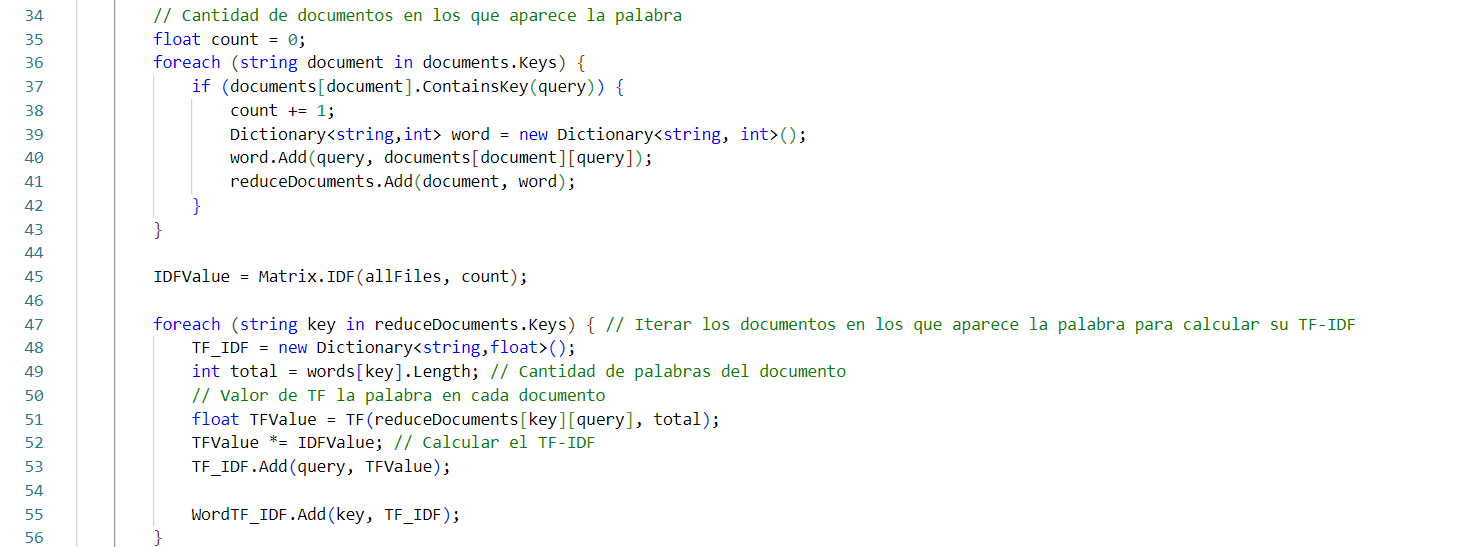
\includegraphics[width=11cm, height=4cm]{fig 1.5.png}\\
	{\tiny Fig. 1.5 Líneas de la clase Matrix de la carpeta MoogleEngine}
\end{center}

En el primer foreach se iteran los documentos para conocer en cuántos aparece la
palabra para calcular después el IDF.Luego, se iteran los documentos seleccionados en los que
sí aparecía la palabra y se calcula el TF en cada uno. Finalmente se calcula la multiplicación,
obteniendo el valor de “relevancia” de la palabra.

\

\textbf{{\large- Moogle}}\\

Esta es la clase principal del programa, donde comienza el proceso de búsqueda. Comienza
en el momento en que se recibe la query. Primeramente, se le hace el mismo “tratamiento”
que a los documentos para que coincidan y exista uniformidad. Además, se implementó una
forma de reconocer si se repiten palabras en la query para reducir el tiempo de la búsqueda, si
existen repeticiones de palabras en la query, solo se calculará su valor de TF-IDF una vez (fig.
1.6).

\begin{center}
	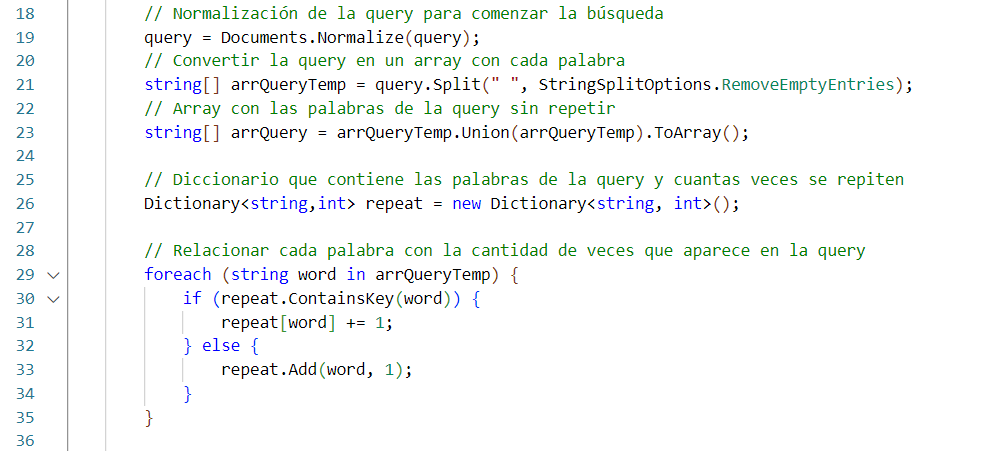
\includegraphics[width=8cm, height=3cm]{fig 1.6.png}\\
	{\tiny Fig. 1.6 Líneas de la clase Moogle de la carpeta MoogleEngine}
\end{center}

Luego de terminado esto, se iteran las palabras sin repetir de la query y se calculan su
TF-IDF en los documentos en los que aparece, pero para conseguir el score por documento se
necesita la suma de estos valores. Para hacerlos coincidir se crearon arrays por cada palabra de
la query de forma tal que se establece una correspondencia entre el orden de los documentos
con los índices. Este array queda de la siguiente manera, si la palabra está contenida en el
documento que se está analizando se encontrará el valor de TF-IDF correspondiente a esa
palabra en ese documento, de forma contraria el valor será 0.
\begin{center}
	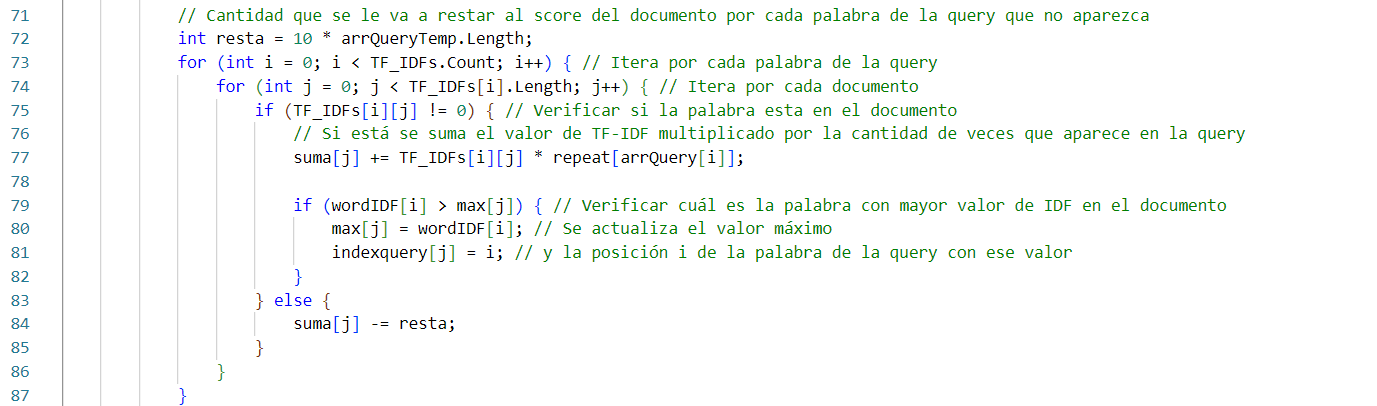
\includegraphics[width=9cm, height=3cm]{fig 1.7.png}\\
	{\tiny Fig. 1.7 Líneas de la clase Moogle de la carpeta MoogleEngine}
\end{center}

Esta forma facilita la suma, sobre todo porque lo interesante es devolver prioritariamente
los documentos que más palabras de la query contenga, así si hay un 0 en la posición del array
será cómodo identificar que el documento no contiene una de las palabras. Si esto pasa, es
conveniente modificar este score para que tenga un valor menor. Además, se aprovecha este
ciclo para reconocer la palabra con mayor valor de IDF por documento para el snippet, como se
había mencionado anteriormente (fig. 1.7).
\

Finalmente, se procede a llenar el array ítems de tipo SearchItem, que contendrá los títulos
de los documentos y los snippets correspondientes, en orden de relevancia acorde a la query
(fig. 1.8).

\begin{center}
	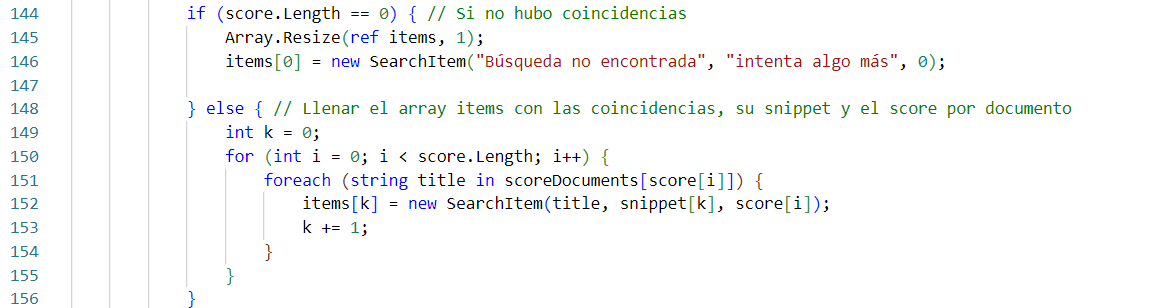
\includegraphics[width=10cm, height=3cm]{fig 1.8.png}\\
	{\tiny Fig. 1.8 Líneas de la clase Moogle de la carpeta MoogleEngine}\\
\end{center}

En el caso excepcional en que la búsqueda sea vacía, es decir, que no se escriba ninguna
palabra se imprimirá esto en pantalla (fig. 1.9).

\begin{center}
	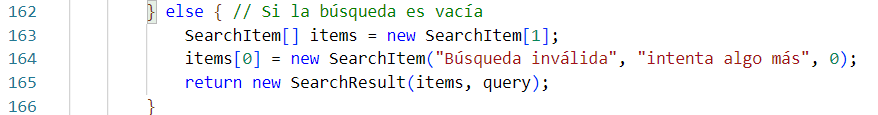
\includegraphics[width=7cm, height=1cm]{fig 1.9.png}\\
	{\tiny Fig. 1.9 Líneas de la clase Moogle de la carpeta MoogleEngine}
\end{center}

\textbf{{\large- SearchItem y SearchResult}}\\
Estas clases estaban implementadas por defecto y permiten el funcionamiento correcto del
programa, las cuales no fueron modificadas. \\

\textbf{{\large- Adicionales}}\\

Adicionalmente, implementé que al devolver los resultados de la búsqueda imprimiera el
tiempo que había tardado la búsqueda, así como los documentos que contienen al menos
una palabra de la query. Además, de que se puede buscar dando click en el botón buscar o
presionando la tecla “enter” (fig. 1.10)
}
\begin{center}
	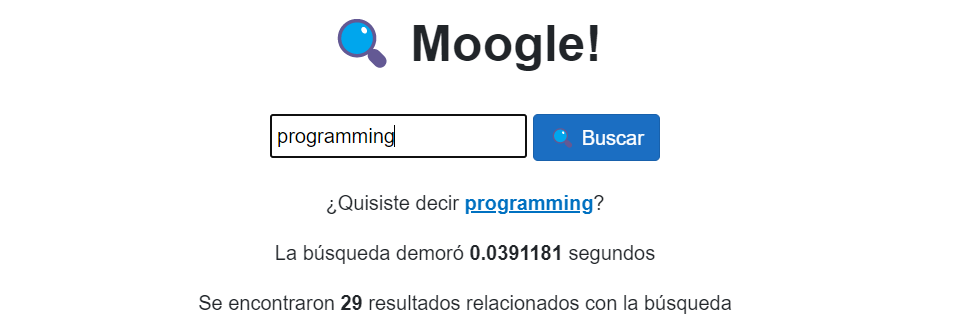
\includegraphics[width=15cm, height=5cm]{fig 1.10.png}\\
	{\tiny Fig. 1.10 Interfaz gráfica del Moogle!}
\end{center}

\end{document}